
\section{Introduction}

In his \emph{Foundations of Arithmetic}, Frege promises ``never to ask for the meaning
of a word in isolation, but only in the context of a proposition''
\parencite*[xvii]{Frege1980}.
This `context principle' is intuitive: words are frequently polysemous, or assume
different connotations and emphasis within different expressions.
Historically, however, contextuality has been a problem for distributional meaning
representations.
Founded on the distributional hypothesis \parencites{Harris1954}{Firth1957}, both
count-based and predictive models of word meaning\footnote{ This terminological
  distinction is due to \textcite{Baroni2014a}.
} originally
produced a single representation for each word in the model's vocabulary.
One of these \emph{static} representations must, therefore, encode all of a word's
senses and connotations, which is an obstacle to its use in modelling context-dependent
phenomena.

Prior to the widespread availability of pre-trained word embeddings
\parencites[e.g.,][]{Mikolov2013}{Pennington2014} and their successors, this problem was
generally addressed by one of two approaches: firstly, by producing a representation
for each sense of a target word and disambiguating between them in the given context
(\emph{word-sense disambiguation}); or secondly, by composing the representation of the
target word with the representations of the words in its context
(\emph{contextualisation}).
These approaches have been largely overshadowed by the advent of model architectures
that take sequences as inputs and naturally produce \emph{contextual} representations
of the items in the sequence, such as Transformers \parencite{Vaswani2017}.

To my knowledge, however, there has been scant direct comparison of the performance of
these contextual representations with the application of prior methods of
contextualisation to static representations.
SemEval-2020 Task 3, ``Graded Word Similarity in Context''
\parencite{Armendariz2020a}, presents an opportunity to make such a comparison.
Briefly, the task is to predict the human judgment of similarity of the same pair of
words in two different contexts (Section~\ref{task-definition}).
I elected to focus on the first subtask, which is to predict the \emph{change} in
similarity, rather than the absolute similarity in each context.
Specifically, I evaluated the results obtained by computing the cosine similarity
between static and contextual embeddings and the composition of these embeddings within
a fixed-size context window.

\section{Task definition}
\label{task-definition}

The first subtask of SemEval-2020 Task 3 is to predict the direction and magnitude of
the change in the human judgment of similarity of the same pair of target words in two
different contexts.
The task is unsupervised: the CoSimLex dataset was used to evaluate the task submissions
but only a minimal `practice kit' of fewer than ten instances was provided in advance.
CoSimLex extends the well-known SimLex-999 dataset \parencite{Hill2015} to include
contexts for each pair in English ($n = 340$), Finnish ($n = 24$), Croatian ($n = 112$),
and Slovene ($n = 111$) \parencite[39-42]{Armendariz2020}.

The score for the first subtask was computed by the uncentered (zero-mean) Pearson
correlation coefficient between the predicted changes in similarity and the human
judgments represented in the CoSimLex dataset \parencite[42]{Armendariz2020}.
This metric is equivalent to the cosine similarity between the two vectors of results:
\begin{equation}
  \text{score}(\vec{\hat{y}}, \vec{y})
  = \frac{\sum_{i = 1}^{n} \hat{y}_i y_i}{\left( \sum_{i = 1}^{n} \hat{y}_i^2 \right)\left( \sum_{i = 1}^{n} y_i^2 \right)}
  = \frac{\vec{\hat{y}} \cdot \vec{y}}{\norm{\vec{\hat{y}}} \norm{\vec{y}}}
\end{equation}
A consequence of this choice of evaluation metric is that composing representations by
addition and their arithmetic mean produce the same results; hence, I elected only to
evaluate the simpler operatoin of addition among the two.

\section{Related work}

Additive composition \parencites[e.g.][]{Kintsch2001}{Mitchell2008}{Mikolov2013a}.
Analysis of the effect of window size on static embeddings.
Analysis of contextual embeddings.

Contextual-embedding models have found broad success on benchmarks that involve language
understanding.
A survey of contextual embeddings is given by \textcite{Liu2020}.
However, as \textcite{Arora2020} point out, these models require significantly greater
computational resources relative to static-embedding models.
THe authors demonstrated that static embeddings `perform surprisingly well' on
named-entity recognition and sentiment analysis tasks when there is adequate training
data and it is linguistically simple.
Furthermore, \textcite{Gupta2019} and \textcite{Bommasani2020} have demonstrated that
static-embeddings can be obtained from contextual-embedding models that outperform
prior static models while retaining their computational advantages.

\section{Methodology}

\begin{figure}
  \label{fig:schematic-procedure}
  \centering
  \captionsetup{justification=centering}
  \newcommand{\period}{.}
  \newcommand*{\orawidest}{accept}
  \newcommand*{\oratallest}{\#\#}
  \newlength{\orawidth}
  \settowidth{\orawidth}{\orawidest}
  \newcommand*{\ora}[1]{\overrightarrow{#1\vphantom{\oratallest}}}
  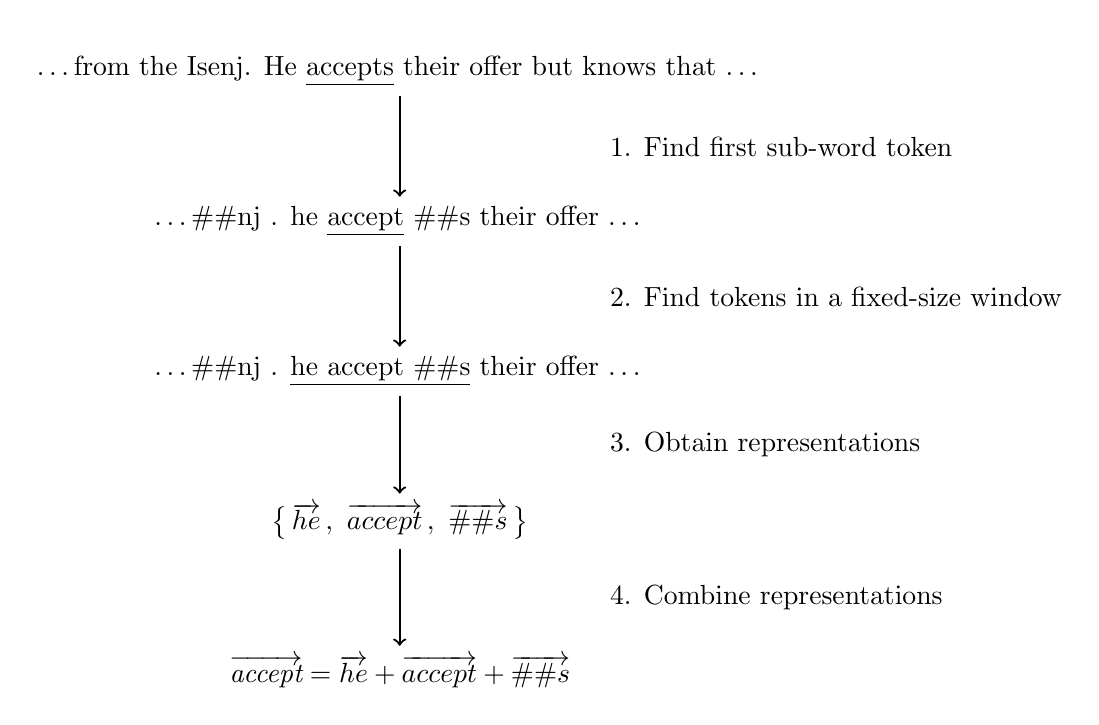
\begin{tikzpicture}[node distance=0.75in]
    \node [label] (a) {\dots from the Isenj\period{} He \underline{accepts} their offer but knows that \dots};
    \node [label, below of=a] (b) {\dots \#\#nj \period{} he \underline{accept} \#\#s their offer \dots};
    \node [label, below of=b] (c) {\dots \#\#nj \period{} \underline{he accept \#\#s} their offer \dots};
    \node [label, below of=c] (d) {$\big\{\,\ora{\text{he}}\,,\ \ora{\text{accept}}\,,\ \ora{\text{\#\#s}}\,\big\}$};
    \node [label, below of=d] (e) {$\ora{\textit{accept}}=\ora{\text{he}}+\ora{\text{accept}}+\ora{\text{\#\#s}}$};
    \draw [thick, ->] (a) -- (b) node[midway, right=1in] {1. Find first sub-word token};
    \draw [thick, ->] (b) -- (c) node[midway, right=1in] {2. Find tokens in a fixed-size window};
    \draw [thick, ->] (c) -- (d) node[midway, right=1in] {3. Obtain representations};
    \draw [thick, ->] (d) -- (e) node[midway, right=1in] {4. Combine representations};
  \end{tikzpicture}
  \caption{A schematic of the procedure used to obtain a contextualised representation
    of a target word from pre-trained static or contextual embeddings. In this example,
    the target word is ``accept'', the window size is three, and the composition
    operation is addition.}
\end{figure}

\begin{figure}
  \label{fig:language-models}
  \centering
  \captionsetup{justification=centering}
  \begin{tabular}{lcccc}
    Model name & English    & Finnish    & Croatian   & Slovene
    \\
    \hline
    \texttt{EMBEDDIA/crosloengual-bert}
               & \checkmark & \checkmark & \checkmark & \checkmark
    \\
    \texttt{bert-base-cased}
               & \checkmark &            &            &
    \\
    \texttt{bert-base-multilingual-cased}
               & \checkmark & \checkmark & \checkmark & \checkmark
    \\
    \texttt{bert-base-multilingual-uncased}
               & \checkmark & \checkmark & \checkmark & \checkmark
    \\
    \texttt{bert-base-uncased}
               & \checkmark &            &            &
    \\
    \texttt{bert-large-cased}
               & \checkmark &            &            &
    \\
    \texttt{bert-large-cased-whole-word-masking}
               & \checkmark &            &            &
    \\
    \texttt{bert-large-uncased}
               & \checkmark &            &            &
    \\
    \texttt{bert-large-uncased-whole-word-masking}
               & \checkmark &            &            &
    \\
    \texttt{classla-bcms-bertic}
               &            &            & \checkmark &
    \\
    \texttt{TurkuNLP/bert-base-finnish-cased-v1}
               &            & \checkmark &            &
    \\
    \texttt{TurkuNLP/bert-base-finnish-uncased-v1}
               &            & \checkmark &            &
    \\
    \texttt{TurkuNLP/bert-large-finnish-cased-v1}
               &            & \checkmark &            &
    \\
  \end{tabular}
  \caption{The pre-trained models available via the HuggingFace \emph{Transformers}
    library \parencite{Wolf2020} that I chose to evaluate for each language.}
\end{figure}

Originally, it would not have been possible to optimise a parameterised model for the
task except by reference to a separate dataset; therefore, I chose to focus on the
application of pre-trained static and contextual embeddings.
The basic procedure of the methods that I evaluated is as follows.
For each pair of target words and each of the two contexts in which they appear, I
obtained a contextualised representation of a target word by:
finding the index of the target word's first sub-word token within the tokens of the target word's context;
finding the tokens within a fixed-size window around the target word's first token;
obtaining the embeddings of the tokens in the window; and
combining the the embeddings to produce a single representation of the target word.

In all cases, the tokenization was performed by and the embeddings were obtained from
pre-trained models available via the HuggingFace \emph{Transformers} library
\parencite{Wolf2020}.
The models that I evaluated for each language are given in Table~\ref{fig:language-models}.
For the static-embedding variants of the procedure, I used the models' input embeddings;
for the contextual-embedding variants, I used the models' outputs.
Several of the submissions to SemEval-2020 Task 3 used a combination of the weights of a
Transformer model's hidden states \parencites[e.g.,][276]{Gamallo2020}[3]{Pessutto2020}[4]{Hettiarachchi2021}; a thorough comparison of the performance of variants
of this approach is beyond the scope of this paper.
Notably, the use of a sub-word vocabulary by these models
\parencite[e.g.,][4174]{Devlin2019} dictates that a target word may be represented by a
different number of tokens in each context.
As a result, the representations of a pair of target words may be different in each
context, even if they are static and the window size is zero.
This explains the non-zero scores obtained by models of this kind
(Section~\ref{appendix:window-size}), particularly for the Finnish language.

Inspired by \textcite{Kintsch2001} and \textcite{Mitchell2008}, I predominantly
investigated the application of element-wise addition and multiplication as composition
operations.
However, preliminary experiments indicated that multiplication performed poorly across
all languages, models, and window sizes; hence, it was discarded before the final
evaluation.
Additionally, I chose to evaluate the concatenation (`stacking') of embeddings.
In the case that the number of embeddings was fewer than the context-window size, i.e.,
the target word was close to the beginning or the end of its context, I right-padded the
concatenated embedding with zeros to obtain contextual embeddings of equal length.

\section{Results}

\subsection{Cost-benefit analysis of contextual embeddings}
\label{sec:cost-benefit}

\subsection{Language-specificity of window-size effects}

Generally, I found that the scores obtained by both static- and contextual-embedding
models were maximised by a non-zero context-window size.
Due to the computational expense of exhaustively searching the possible window sizes,
I applied a heuristic to constrain the search space.
A naïve estimation of the average number of words in each context, i.e., segmenting on
whitespace, gave a result of between $40$ and $60$ for the different languages.
Therefore, for the static-embedding models, I chose $50$ as an upper bound on the
window size.
The motivation to choose a smaller maximum window size for contextual-embedding models
was similarly economical (Section~\ref{sec:cost-benefit}); however, as the window size
approaches the length of the sequence, one would expect a combination of token
representations to be superseded by the sequence-level representation of the model,
e.g., the special \texttt{CLS} token of BERT variants \parencite[4174]{Devlin2019}.
These heuristics were largely vindicated by the results of the evaluation, which
demonstrated that the scores decrease as the window size approaches the maximum.

The influence of the window size is intuitive in the case of static embeddings.
Without a context window, the representations of a target word only differ between
expressions if the word is represented by different sub-word tokens in the different
expressions.
A similar argument applies to contextual embeddings, in that a target word may be
represented by multiple sub-word tokens.
The window sizes that maximise the score for each language and model are given in
Table~\ref{table:best-window-size}.

\section{Discussion}

\textcite{Batchkarov2016} critically analyse word similarity as an evaluation
methodology for distributional semantic models.
In particular, the notion of `similarity' manifested by these models encompasses a
broad range of semantic relations \parencite[e.g.,][2]{Pado2003}, with the consequence
that performance on an intrinsic word-similarity task does not necessarily translate
to extrinsic downstream tasks \parencite[7-8]{Batchkarov2016}.
Moreover, inter-annotator agreement is generally poor for word-similarity tasks in
comparison to more specific downstream tasks \parencite[8-9]{Batchkarov2016}.

\section{Conclusion}

In this paper, I have presented the results of a hypothetical submission to SemEval-2020
Task 3, ``Graded Word Similarity in Context''.
The purpose of this evaluation was to compare the performance of static and contextual
embeddings and their composition within a fixed-size context window on the task of
predicting the change in the human judgment of similarity of a pair of words in two
different contexts.
I found that contextual embeddings generally outperformed static embeddings, but at a
significant computational cost, and that composition benefited both static and
contextual embeddings of sub-word tokens, with highly language-specific dependence
on the window size.

The results that I have given must be interpreted in context: the original submission
authors did not have access to the evaluation dataset prior to submitting their results,
only the `practice kit' of very few instances, and were therefore unable to optimise a
parameter such as the window size prior to submission.
With this caveat, I achieved several notable results:
\begin{itemize}
  \item The contextual embeddings of \texttt{EMBEDDIA/crosloengual-bert} with a window
        size of three would have placed second among the Croatian submissions
        ($0.708$).
  \item The contextual embeddings of \texttt{TurkuNLP/bert-base-finnish-uncased-v1} with
        a window size of zero would have placed fourth among the Finnish submissions
        ($0.679$).
  \item The \emph{static} embeddings of \texttt{TurkuNLP/bert-base-finnish-uncased-v1}
        with a window size of zero outperform several of the Finnish submissions,
        including the baseline ($0.564$).
\end{itemize}
Given the significant expense of applying contextual-embedding models, these results
highlight the importance of analysing the complexity of the task at hand and considering
the possibility that a simpler model produces adequate results.